\documentclass[11pt]{article}
\usepackage[margin=1in,footskip=0.25in]{geometry}

%\usepackage{helvet}
%\renewcommand{\familydefault}{\sfdefault}
\renewcommand\refname{\vskip -1cm}
%\renewcommand{\rmdefault}{phv} % Arial
%\renewcommand{\sfdefault}{phv} % Arial
\usepackage{setspace}
\usepackage{wrapfig}
\usepackage{amsmath}
\usepackage{amssymb}
\usepackage{graphicx}
\usepackage{mathrsfs}
\usepackage{bm}
\usepackage{wasysym}
\usepackage{placeins}
\usepackage{multirow}
\usepackage[T1]{fontenc}
\usepackage[super]{natbib}
\usepackage{framed}
\usepackage{caption}
\usepackage{longtable}




\begin{document}

\title{The effect of starvation on the dynamics of consumer populations}
\maketitle


\section{Introduction}
%Focus on the tradeoff between REPRODUCTION AND SURVIVAL AS A FUNCTION OF ENERGETIC STATE

The behavioral ecology of most, if not all, organisms is influenced by the energetic state of individuals from which the population is composed.
An individual's energetic state, which can range from starving (energetically defficient) to satiated (energetially replete), directly influences how it invests its stores in an uncertain environment.
Such state-dependent behaviors are generally manifested as trade-offs.
A major trade-off that we consider in detail concerns reproductive vs. non-reproductive energetic investment strategies.
As has been shown in [examples], individuals that are energetically deficient are unable to invest energy stores towards reproduction.
Among sexually reproducing species, even when reproduction occurs, the offspring is often naturally aborted if there is not sufficient caloric resources available to the parent.

Here we explore how reproductive trade-offs, which occur at the level of the individual, may influence the dynamics of a population of individuals.
We first establish a simple stage-structured population model that captures the essential elements of energetic reproductive tradeoffs, and explore how the rate of starvation impacts dynamics at the level of the population.
We then develop a more general model in order to understand if there are common attriburtes of these dynamics that have implications beyond the simple stage-structured model.
Finally, we compare our population-dynamic approach with a stochastic dynamic program that incorporates different individual-level behaviors as a function of energetic state.



\section{Methods}
\subsection{Model description}

We first integrate energetics into the dynamics of a consumer-resource system by assuming that the consumer population can be divided into discrete energetic states, the occupation of each being contingent on the consumption of a single resource $R$.
In the simplest case, there are only two energetic states for the consumer population: \emph{i}) an energetically replete state $F$, where the consumer reproduces at rate $\lambda$, and \emph{ii}) an energetically deficient state $H$, where reproduction is suppressed, and mortality occurs at rate $\mu$.
Consumers transition from state $F$ to state $H$ by starvation at rate $\sigma$ and in proportion to the lack of food $1-R$.
Conversely, consumers recover from state $H$ to the energetically replete state $F$ at rate $\rho$ and in proportion to the density of resources consumed $R$.
The resource has logistic growth with a linear growth rate $a$ and a carrying capacity of unity.
Resources are eliminated by the consumer in either state: by energetically deficient consumers at rate $\rho$, and by energetically replete consumers at rate $b$.
Accordingly, the system of equations is written

\begin{align}
\frac{\rm d}{\rm dt} F &= \lambda F + \rho HR - \sigma (1-R)F, \nonumber \\
\frac{\rm d}{\rm dt} H &= \sigma (1-R)F - \rho RH - \mu H, \nonumber \\
\frac{\rm d}{\rm dt} R &= a R(1-R) - R(\rho H+ b F).
\end{align}

There are three steady states for the 2-stage consumer-resource system: two trivial steady states at $(R^*=0,H^*=0,F^*=0)$ and $(R^*=1,H^*=0,F^*=0)$, and one non-trivial internal steady state where $(R^*>0,H^*>0,F^*>0)$.
The latter steady state is the one of chief ecological interest, where

\begin{align}
F^* &= \frac{a  \lambda  \mu  (\mu +\rho )}{(\lambda  \rho +\mu  \sigma ) (\lambda  \rho +\mu  m)}, \nonumber \\
H^* &= \frac{a  \lambda ^2 (\mu +\rho )}{(\lambda  \rho +\mu  \sigma ) (\lambda  \rho +\mu  m)}, \nonumber \\
R^* &= \frac{\mu  (\sigma -\lambda )}{\lambda  \rho +\mu  \sigma }.	
\end{align}

\noindent Because there is only one internal steady state, as long as it is stable the population trajectories will be globally attracted to it for any set of initial conditions greater than zero.

Analysis of the stability of the consumer-resource system is explored with respect to the local stability of the internal steady state, which is the only feasible steady state as long as both the consumer and resource have non-zero, positive, values.
In a multidimensional system, linear stability is determined with respect to the Jacobian Matrix $\bf J$, which is a matrix where each element is defined by the partial derivative of each equation with respect to each variable.
In the case of the 2-stage consumer model, the Jacobian evaluated at the internal steady state (denoted by $|_*$) is written

\begin{equation}
\mathbf{J}|_* =
%\left(
%\begin{array}{ccc}
% -F^* m+(1-R^*) a -R^* a -H^* \rho  & -R^* \rho  & -m R^* \\
% -H^* \rho -F^* \sigma  & -\mu -R^* \rho  & (1-R^*) \sigma  \\
% H^* \rho +F^* \sigma  & R^* \rho  & \lambda -(1-R^*) \sigma  \\
%\end{array}
%\right).
\left(
\begin{array}{ccc}
 \frac{\lambda  \rho  (\lambda -\sigma )}{\lambda  \rho +\mu  \sigma } & \frac{\mu  \rho  (\sigma -\lambda )}{\lambda  \rho +\mu  \sigma } & \frac{\alpha  \lambda  (\mu +\rho )}{m \mu +\lambda  \rho } \\
 \frac{\lambda  (\mu +\rho ) \sigma }{\lambda  \rho +\mu  \sigma } & -\frac{\mu  (\mu +\rho ) \sigma }{\lambda  \rho +\mu  \sigma } & -\frac{\alpha  \lambda  (\mu +\rho )}{m \mu +\lambda  \rho } \\
 \frac{m \mu  (\lambda -\sigma )}{\lambda  \rho +\mu  \sigma } & \frac{\mu  \rho  (\lambda -\sigma )}{\lambda  \rho +\mu  \sigma } & \frac{\alpha  \mu  (\lambda -\sigma )}{\lambda  \rho +\mu  \sigma } \\
\end{array}
\right).
\end{equation}


%Transcritical bifurcation
If the parameters of the Jacobian matrix at the internal steady state are such that its leading eigenvalue is $<0$, then the system is stable to small pulse perturbations, conditioned on the value of the starvation rate $\sigma$ relative to the value of the consumer reproduction rate $\lambda$.
As $\sigma$ nears and becomes lower than a given $\lambda$, the resource steady state $R^*$ crosses the origin and exchanges stability to become unstable.
As such, a transcritical bifurcation exists at $\lambda = \sigma$, such that the existence of an internal stable fixed point is dependent on the condition that $\sigma > \lambda$.
Biologically, this means that the rate of starvation is greater (operating on a smaller timescale) than the rate of consumer reproduction (operating on a relatively longer timescale).
As will be shown in Section XX, this general expectation will hold for most classes of organisms, while the exact difference in timescales between reproduction and starvation can be derived using allometric scaling relationships.
%Kempes (REF) has shown that population growth rates scale to $M^{\alpha-1}$ (where $M$ is the reproductive mass of an organism and $\alpha$ is the scaling exponent), whereas starvation is necessarily bound to shorter timescales, which will be elaborated on below.


%Hopf bifurcation
Oscillating, or cyclic, dynamics presents additional risks to a population.
If the cycles are large, or have regions where low values are attained, 

Of additional interest is the existence of parameter regions that permit the existence of oscillatory, or cyclic, dynamics.
Cycles arise when a pair of complex conjugate eigenvalues cross the imaginary axis and attain positive real parts.
This condition is called a Hopf bifurcation, and is defined by ${\rm Det}({\bf S}) = 0$, where $\bf S$ is the Sylvester matrix, which is composed of the coefficients of the characteristic polynomial describing the Jacobian matrix.
Although the Hopf condition for the specific 2-stage model cannot be easily solved, it can be explored using a symbolic computational language such as \emph{Mathematica}.

%What parameters is the Hopf bifurcation primarily dependent on?

%The natural ordering of the scaled rates
%lambda < rho < sigma
%if lambda is 0.2, and sigma is 0.8, then rho is between 0.2 and 0.8.
%In other words, lambda has the SLOWEST timescale, sigma has the fastest timescale, and rho has a timescale intermediate to both.


\subsection{Analysis of a generalized model}

$\xi$ ~~ $\zeta$

\subsection{Allometric scaling relationships}


\section{Results}

To determine how the consumer-resource system impacted by different rates of starvation, we analyze the systems with respect to $p$.


\section{Discussion}

%The reproductive tradeoff as a strategy
%
% \begin{figure}[h]
% 	\centering
% 	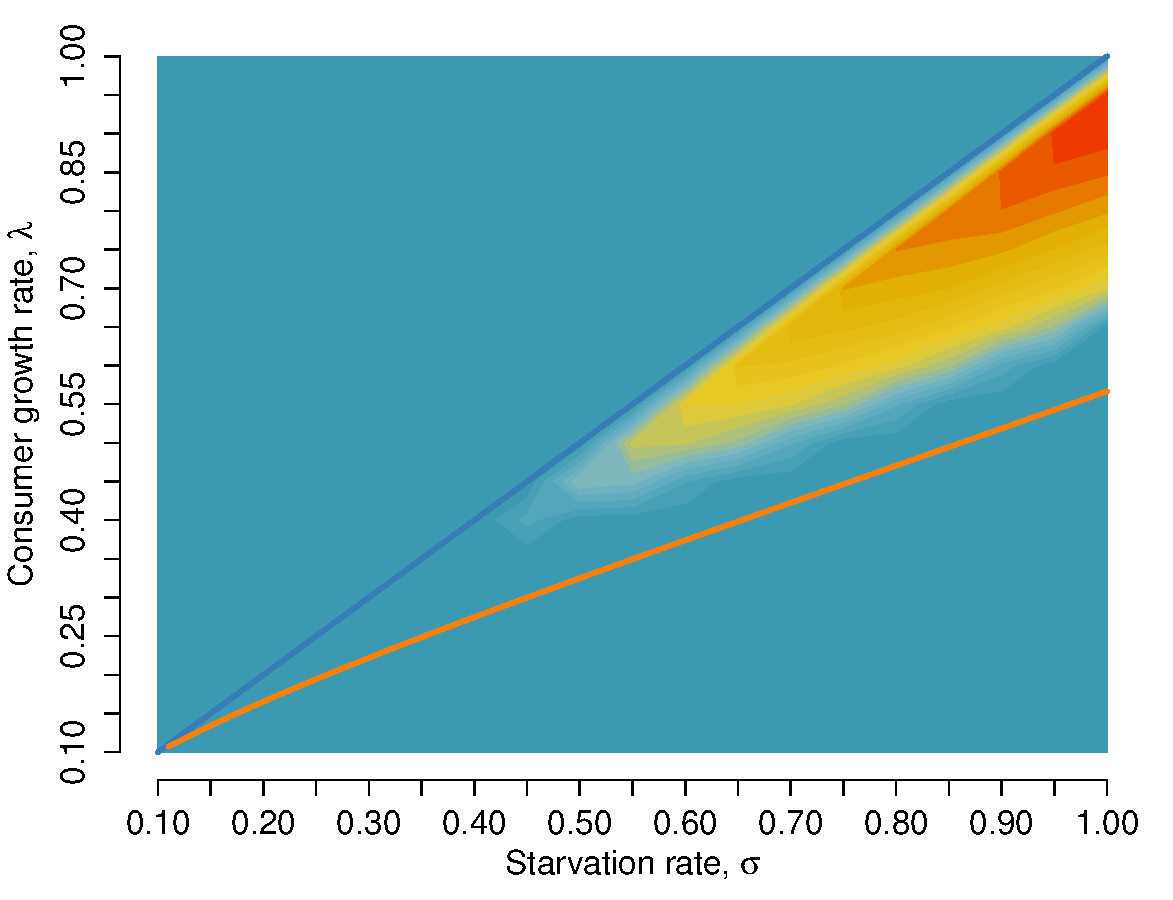
\includegraphics[width=0.5\textwidth]{fig_Hopf.pdf}
% 	\caption{
% 	Saddle Node bifurcation
% 	}
% 	\label{SN}
% \end{figure}
%
%
% \begin{figure}[h]
% 	\centering
% 	\includegraphics[width=0.5\textwidth]{fig_resvuln.pdf}
% 	\caption{
% 	Probability that the resource value is less than threshold = 0.05
% 	}
% 	\label{SN}
% \end{figure}
%
%
%
% \begin{figure}[h]
% 	\centering
% 	\includegraphics[width=0.5\textwidth]{fig_Competition.pdf}
% 	\caption{
% 	Hopf bifurcation
% 	}
% 	\label{SN}
% \end{figure}






\end{document}
